\section{Geometría}

\begin{questions}
\question
    Un sastre pretendía cortar de un pedazo
de tela un mantel de cierta área y de forma
cuadrada, pero no fue posible obtenerlo así.
Por esto, decidió cortarlo en forma rectangular,
de tal manera que tuviera por ancho el lado del
cuadrado disminuido en 2 y por largo el lado del
cuadrado aumentado en 2.

Entonces, el área del mantel rectangular resultó
con respecto a la del cuadrangular \footnote{\cite{SEMA2021}}

\begin{choices}
    \choice igual.
    \choice 2 unidades cuadradas menor.
    \CorrectChoice 4 unidades cuadradas menor. %%%%%%%
    \choice 2 unidades cuadradas mayor.
    \choice 4 unidades cuadradas mayor.
\end{choices}

\begin{solution}
Dibujemos el trozo de tela del sastre. Punteado era el deseo original, y el de la línea continua fue el que terminó haciendo. 
    \begin{center}
    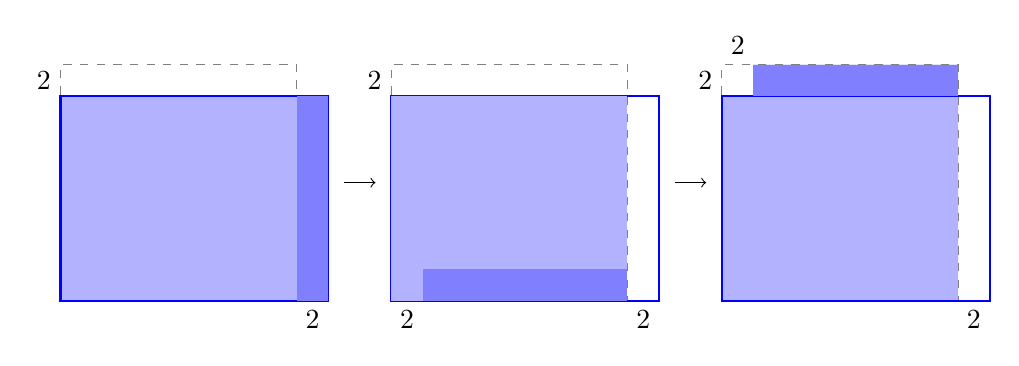
\begin{tikzpicture}
        \draw[gray, dashed] (0,0) -- (3,0) -- (3,3) -- (0,3) -- cycle;
        \draw[blue, fill=blue!30, thick] (0,0) -- (3.4, 0) -- (3.4, 2.6) -- (0, 2.6) -- cycle; 
        \node[below] at (3.2,0) {2};
        \node[left] at (0,2.8) {2};
        \fill[color=blue!50] (3,0) rectangle (3.4, 2.6);
        \draw[->] (3.6, 1.5) -- (4, 1.5);
        \begin{scope}[xshift=4.2cm]
        \draw[gray, dashed] (0,0) -- (3,0) -- (3,3) -- (0,3) -- cycle;
        \draw[blue, thick] (0,0) -- (3.4, 0) -- (3.4, 2.6) -- (0, 2.6) -- cycle; 
        \fill[blue!30] (0,0) rectangle (3,2.6);
        \node[below] at (3.2,0) {2};
        \node[below] at (0.2,0) {2};
        \node[left] at (0,2.8) {2};
        \fill[color=blue!50] (3,0) rectangle (0.4, 0.4);
        \end{scope}
        \draw[->, xshift=4.2cm] (3.6, 1.5) -- (4, 1.5);
        \begin{scope}[xshift=8.4cm]
        \draw[fill = blue!30, draw=gray, dashed] (0,0) -- (3,0) -- (3,3) -- (0.4,3) -- (0.4, 2.6) -- (0,2.6) -- cycle;
        \draw[gray, dashed] (0,0) -- (3,0) -- (3,3) -- (0,3) -- cycle;
        \draw[blue, thick] (0,0) -- (3.4, 0) -- (3.4, 2.6) -- (0, 2.6) -- cycle; 
        \node[below] at (3.2,0) {2};
        \node[above] at (0.2,3) {2};
        \node[left] at (0,2.8) {2};
        \fill[color=blue!50, yshift=2.6cm] (3,0) rectangle (0.4, 0.4);
        \end{scope}
    \end{tikzpicture}
    \end{center}

    Vemos entonces que el trozo de tela que terminó cortando el sastre es un poco más pequeño que el cuadrado original. De hecho, es más pequeño por $2\cdot 2 = 4$ unidades cuadradas, el cuadradito que le falta en la tercera figura para completar todo el cuadrado.

    Algebraicamente, tenemos que si $l$ es el lado del cuadrado, entonces el área del cuadrado original es de $l^2$. Por otro lado el ancho del rectángulo que terminó cortando es de $l-2$ y su largo $l+2$, de forma que su área es de 
    \[
    (l-2)(l+2) = l\cdot l + l\cdot 2- 2\cdot l - 2\cdot 2 = l^2+2l-2l -4 = l^2-4.
    \]
    Es decir, 4 unidades cuadradas menos que el cuadrado original. La respuesta correcta es la B.

    Este es un ejemplo de la fórmula notable ``diferencia de cuadrados:''
    \[(a+b)(a-b) = a^2-b^2\] \hfill $\square$
\end{solution}


\question
    Un cuadrilátero $P$ tiene 32 cm de perímetro
y 48 $\cmdos$ de área. Un cuadrado $Q$ posee un
perímetro igual a la cuarta parte del perímetro
del cuadrilátero $P$.

¿Cuál es la diferencia entre las áreas del
cuadrilátero $P$ y el cuadrado $Q$? \footnote{\cite{SEMA2021}}

\begin{choices}
    \choice 12 $\cmdos$
    \choice 23 $\cmdos$
    \choice 28 $\cmdos$
    \choice 39 $\cmdos$
    \choice 44 $\cmdos$
\end{choices}

\begin{solution}
    El perímetro del cuadrado $Q$ es de
    \[P_Q = \frac{1}{4}P_P = \frac{1}{4}32\cm = 8\cm\]
    Donde $P_F$ representa el perímetro de una figura $F$ (en este caso $F$ se cambia por el cuadrilátero $P$ o por el cuadrado $Q$). Como todos los lados son iguales, el lado $l$ del cuadrado mide la cuarta parte del perímetro $l = 8\cm/4 = 2\cm$. Y por tanto, el área del cuadrado es de $A_Q=l^2 = 2^2\cmdos = 4\cmdos$. La diferencia entre las áreas de $P$ y $Q$ es de
    \[
    A_P - A_Q = 48\cmdos-4\cmdos = 44\cmdos
    \]
    Donde usamos la misma idea, $A_F$ es el área de la figura $F$ ($P$ o $Q$). La respuesta correcta es la E. \hfill $\square$
\end{solution}

\question
Un terreno rectangular tiene un perímetro de $60$ metros y el largo es el doble del ancho. ¿Cuánto mide el ancho?

\begin{choices}
    \choice 10 m %%%
    \choice 12 m
    \choice 15 m
    \choice 18 m
\end{choices}

\begin{solution}
    Hagamos una figura
    \begin{center}
    \begin{tikzpicture}
        \draw (0,0) -- node[below] {$2x$} (4,0) -- node[right] {$x$} (4,2) -- node[above] {$2x$} (0,2) -- node[left] {$x$} cycle;
    \end{tikzpicture}
    \end{center}
    Aquí pusimos $x$ al ancho y por tanto el largo es $2x$. Tenemos entonces que el perímetro es la suma de todos los lados $P = x + 2x + x + 2x = 6x$ y es igual a 60 metros. Por tanto el ancho mide $x = 60/6 = 10$ metros. La respuesta correcta es la A. \hfill $\square$
\end{solution}

\question
La altura de un triángulo es el doble de su base. Si el área del triángulo es $144 \cmdos$, ¿cuánto mide su base?

\begin{choices}
    \choice 6 cm
    \choice 8 cm
    \choice 9 cm
    \choice 12 cm %%%
\end{choices}

\begin{solution}
    De nuevo hacemos una figura para orientarnos
    \begin{center}
    \begin{tikzpicture}
        \draw (0,0) -- node [below] {$b$} (2,0) -- (-1, 4) -- cycle;
        \draw[dashed] (0,0) -- (-1,0) -- node[left]{$h= 2b$} (-1,4);
        \draw (-1,0) rectangle (-0.8,0.2);
    \end{tikzpicture}
    \end{center}

    El área sabemos que es
    \[
    A = 144\cmdos =  \frac{b\cdot h}{2} = \frac{b \cdot 2b}{2} = b^2
    \]
    Sabemos que $144 = 12^2$ (vale la pena repasar cuáles son los cuadrados perfectos, al menos hasta 15), luego la base del triángulo mide $b=12\cm$

    Como una curiosidad, podemos obtener un cuadrado de lado $b$ a partir de este triángulo:
    \begin{center}
    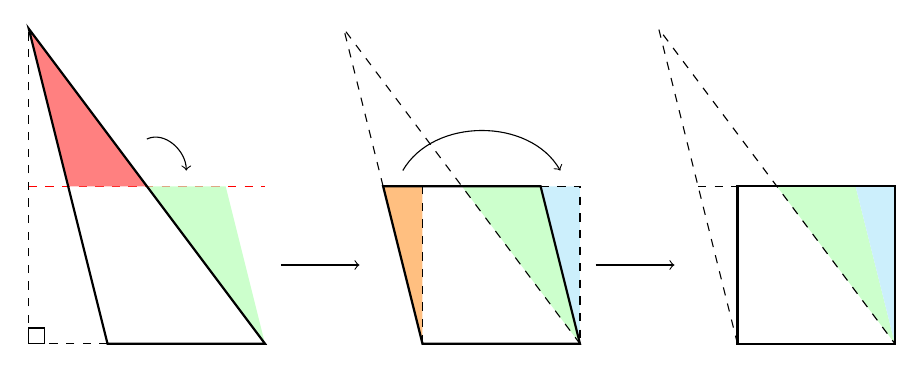
\begin{tikzpicture}
        \draw[dashed] (0,0) -- (-1,0) -- (-1,2) -- (-1,4);
        \draw (-1,0) rectangle (-0.8,0.2);
        \draw[red, dashed] (-1,2) -- (2, 2);
        \fill[red!50] (-0.5, 2) -- (0.5,2) -- (-1,4) -- cycle;
        \fill[green!20] (0.5,2) -- (1.5, 2) -- (2, 0) -- cycle;
        \draw[->] (0.5, 2.6) to [out=25, in=90] (1, 2.2);
        \draw[thick] (0,0) -- (2,0) -- (-1, 4) -- cycle;
        \draw[->] (2.2, 1) -- (3.2, 1);
        \begin{scope}[shift = {(4, 0)}]
            \fill[fill=orange!50] (0, 2) -- (0,0) -- (-0.5,2) -- cycle;
            \draw[dashed] (0,0)-- (0,2);
            \draw[->] (-0.25,2.2) to [out= 60, in=120] (1.75,2.2);
            \fill[fill=green!20] (2,0) -- (1.5, 2) -- (0.5,2) -- cycle;
            \fill[fill=cyan!20] (2,0) -- (1.5, 2) -- (2,2) -- cycle;
            \draw[dashed] (1.5, 2) -- (2,2) -- (2,0);
            \draw[dashed] (-0.5,2) -- (-1,4) -- (2,0);
            \draw[thick] (0,0) -- (2,0) -- (1.5,2) -- (-0.5,2) -- cycle;
        \end{scope}
        \draw[->] (6.2, 1) -- (7.2, 1);
        \begin{scope}[shift={(8,0)}]
            \fill[fill=green!20] (2,0) -- (1.5, 2) -- (0.5,2) -- cycle;
            \fill[fill=cyan!20] (2,0) -- (1.5, 2) -- (2,2) -- cycle;
            \draw[dashed] (0,0) -- (-1,4) -- (2,0);
            \draw[dashed] (-0.5,2) -- (0,2);
            \draw[thick] (0,0) rectangle (2,2);
        \end{scope}
    \end{tikzpicture}
    \end{center} \hfill $\square$
\end{solution}

\question
En Papa John's venden pizzas de 8 pulgadas y de 10 pulgadas de diámetro. Si la pizza grande cuesta 5000 colones y la pequeña 4000, el precio por pulgada cuadrada de la pizza pequeña es

\begin{choices}
    \CorrectChoice 25 \% más que el de la pizza grande. %%%%%%%
    \choice 10 \% más que el de la pizza grande.
    \choice 10 \% menos que el de la pizza grande.
    \choice El mismo que el de la pizza grande.
\end{choices}

\begin{solution}
    Primero, note que nos preguntan el precio por \textbf{pulgada cuadrada}, una medida de área. Por tanto, necesitamos medir el área de las pizzas. El radio de la pizza pequeña es de $8/2 = 4$ pulgadas y el de la grande es $10/2 = 5$ pulgadas. Así, sus áreas son
    \[
    A_p = \pi\cdot4^2 \operatorname{in}^2 = 16\pi \operatorname{in}^2 \quad A_g = \pi\cdot 5^2 \operatorname{in}^2 = 25\pi \operatorname{in}^2
    \]
    Calculando el precio por pulgada cuadrada, el de la pizza pequeña es $4000/(16\pi) = 1000/(4\pi) = 250/\pi$ colones por pulgada cuadrada y el de la grande es $5000/(25\pi) = 1000/(5\pi) = 200/\pi$. Por tanto, para calcular el porcentaje del precio por pulgada cuadrada de la pizza pequeña relativo al de la pizza grande, dividimos:
    \[
    \frac{250/\pi}{200/\pi} = \frac{250}{200} = \frac{25}{20} = \frac{5}{4} = 1.25 = 125\%.
    \]
    Es decir, el precio por pulgada cuadrada de la pizza pequeña es un $25\%$ más que el de la pizza grande.
    
    (Aunque no lo parezca, con aumentar un $25\%$ el diámetro de una pizza, el área aumenta en más del $50\%$, de hecho, va a ser $1.25^2 = 1.5625$ veces el área de la pequeña, un $56\%$ más). \hfill $\square$
\end{solution}

\question El largo de un terreno rectangular es el doble de su ancho. Si el terreno tiene un área de $288$ metros cuadrados, ¿cuál es su largo?
\begin{choices}
    \choice 12 m
    \CorrectChoice 24 m
    \choice 36 m
    \choice 96 m
\end{choices}

\begin{solution}
    Hacemos un dibujo
    \begin{center}
    \begin{tikzpicture}
        \draw (0,0) -- node[below] {$2x$} (4,0) -- (4,2) -- (0,2) -- node[left] {$x$} cycle;
        \draw[dashed] (2,0) -- (2,2);
        \node at (1,1) {$x^2$};
        \node at (3,1) {$x^2$};
        
    \end{tikzpicture}
    \end{center}
    Si $x$ es el ancho del terreno, $2x$ es el largo y su área es $288\text{m}^2 = 2x^2$, por lo que $x^2 = 144 \text m^2$. De esta forma $x = 12$ m. El largo del terreno es, por tanto $2x = 24$ m. \hfill $\square$
\end{solution}

\question André, asumiendo que su finca tenía forma cuadrada, midió uno solo de los lados y obtuvo que medía 120 m. Daniel midió ambos lados de la finca y, en el lado que midió André, Daniel obtuvo una medida 10\% menor que la de André. Al medir el otro lado, obtuvo un 20\% más que con el primero. Ambos calculan el área que piensan que tiene la finca. Con certeza
\begin{choices}
    \choice Obtienen áreas iguales
    \choice El área obtenida por Daniel es mayor que la obtenida por André.
    \CorrectChoice El área obtenida por André es mayor que la obtenida por Daniel.
    \choice No hay suficiente información para responder.
\end{choices}

\begin{solution}
    Si L es el lado que midió André, este obtuvo $120$ metros y Daniel obtuvo un $10 \%$ menos, es decir el $90\%$, que es $0.9 \cdot 120 = 9\cdot 12 = 90 + 18 = 108$ metros. Después midió el segundo lado y obtuvo un $20\%$ más que con el primero, es decir, un $120\%$ de $108$, que sería $1.2\cdot 108 = 1.2\cdot100 + 1.2\cdot 8 = 120 + 9.6 = 129.6$ metros. Ahora podemos calcular las áreas que obtuvo cada uno.

    Como André asumió que era cuadrada, obtuvo un área de (en metros cuadrados ambas)
    \[
    120\cdot120 = 12 \cdot 12 \cdot 100 = 14400
    \]
    y Daniel una de
    \[
    108 \cdot 129.6 = 100\cdot 129.6 + 8\cdot 129.6 = 12960 + 800+160 + 72 +4.8 = 13760+236.8 = 13996.8
    \]
    Por tanto con certeza André obtuvo un área mayor que la de Daniel. 

    Duramos mucho haciendo cálculos. Que pasa si olvidamos la medida de $120$ m, y simplemente decimos que $x$ fue la medida obtenida por André, entonces podemos simplificarlo todo.

    El área obtenida por André fue de $x^2$, y Daniel obtuvo, para el lado que midió André, $0.9x$ (un $10\%$ menos), y con el otro, un $20\%$ más que $0.9x$, es decir $1.2\cdot 0.9x$. Así el área que obtiene Daniel es de $0.9x\cdot 1.2\cdot0.9x = 0.9^2\cdot1.2x^2$ . Para ver si $0.9^2\cdot1.2x^2 $ es mayor o menor que $x^2$, basta ver si $0.9^2\cdot1.2$ es mayor o menor que 1, pues $x^2$ es un número positivo.
    \[
    0.9^2\cdot 1.2 = \left(\frac{9}{10}\right)^2\cdot\frac{12}{10} = \frac{81\cdot 12}{100\cdot 10} = \frac{810+162}{1000} = \frac{972}{1000} < 1
    \]
    Y con bastantes menos cálculos, obtenemos que la medida que obtuvo Daniel es menor (¿en qué porcentaje?) que la que obtuvo André. \hfill $\square$
\end{solution}

\question En la figura se muestra un círculo inscrito en un cuadrado cuyo perímetro es 32 cm. El área, en centímetros cuadrados, de la región sombreada con gris corresponde a
\begin{center}
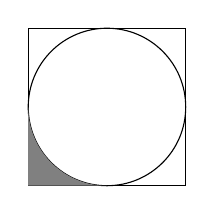
\begin{tikzpicture}
    \draw (-1, -1) rectangle (1, 1);
    \draw (0,0) circle [radius=1cm];
    \fill[gray] (-1, -1) -- (0, -1) arc[start angle=-90, end angle=-180, radius =1cm] -- cycle;
\end{tikzpicture}
\end{center}
\begin{choices}
    \choice $12\pi$
    \CorrectChoice $16-4\pi$
    \choice $64-4\pi$
    \choice $4\pi - 8$
\end{choices}

\begin{solution}
    Note que el área sombreada es una de las cuatro esquinas que quedan del cuadrado al quitar el círculo inscrito. Por tanto, una forma de calcularla es calculando el área del cuadrado, restando la del círculo y dividiendo entre 4. Eso vamos a hacer a continuación.

    Como el perímetro de un cuadrado es la suma de los cuatro lados, $4l = 32$cm, y por tanto $l=8$cm. De aquí, tenemos que el área del cuadrado es $A_\square = l^2 = 8^2\cmdos = 64\cmdos$. 
    
    Por otro lado, notemos que el diámetro del círculo coincide con el lado del cuadrado, 8cm. El radio es la mitad, $r = 8/2 = 4$cm. El área del círculo es entonces $A_\bigcirc = \pi\cdot r^2 = 16\pi\cmdos$
    
    Por tanto, el área de lo que queda al quitar el círculo al cuadrado es $64-16\pi$ centímetros cuadrados. Esta área está formada por cuatro esquinas (
\begin{tikzpicture}[scale = 0.2]
    \draw (-1, -1) rectangle (1, 1);
    \draw (0,0) circle [radius=1cm];
    \fill[gray] (-1, -1) -- (0, -1) arc[start angle=-90, end angle=-180, radius =1cm] -- cycle;
    \fill[gray!50] (-1, 1) -- (1, 1) -- (1, -1) -- (0,-1) arc[start angle=-90, end angle=180, radius =1cm] -- cycle;
\end{tikzpicture}) como la que queremos calcular, por lo que el área sombreada es (en centímetros cuadrados)
    \[
    A_S = \frac{64-16\pi}{4} = \frac{64}{4} - \frac{16\pi}{4} = 16 - 4\pi
    \]
La respuesta correcta es la B.
\end{solution} 

\question En la figura adjunta se muestra un \textit{pentaminó}, que es una figura compuesta por 5 cuadrados congruentes en donde cada uno tiene al menos un lado en común con otro cuadrado. Si el perímetro de la figura es de 60 cm, entonces el área de la región sombreada con gris, en centímetros cuadrados, corresponde a
\begin{center}
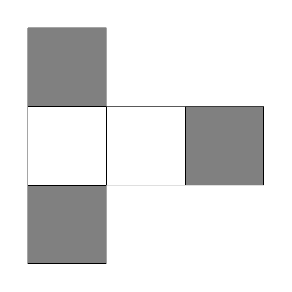
\begin{tikzpicture}
    \clip (0,0) -- (1,0) -- (1,1) -- (3,1) -- (3,2) -- (1, 2) -- (1,3) -- (0,3) -- cycle;
    \fill[gray] (0,0) rectangle (1,1);
    \fill[gray] (0,2) rectangle (1,3);
    \fill[gray] (2,1) rectangle (3,2);
    \draw (0,0) grid (3,3);
\end{tikzpicture}
\end{center}

\begin{choices}
    \choice 25
    \choice 27
    \choice 36
    \choice 75
\end{choices}

\end{questions}
